\documentclass[tikz,border=12pt]{standalone}
\usepackage[T1]{fontenc}
\usepackage{mathpazo}
\usepackage{amsmath,amssymb}
\usetikzlibrary{arrows.meta, positioning, calc, fit, decorations.pathreplacing}

\definecolor{stblue}{HTML}{7B97AD}
\definecolor{rwgold}{HTML}{B8995E}
\definecolor{sage}{HTML}{7A9A7E}
\definecolor{dkbrown}{HTML}{3D3530}
\definecolor{wmgray}{HTML}{7B7067}
\definecolor{cream}{HTML}{F9F6F0}
\definecolor{border}{HTML}{D4C9B8}
\definecolor{terracotta}{HTML}{C47A6A}
\definecolor{lavender}{HTML}{907EA0}

\begin{document}
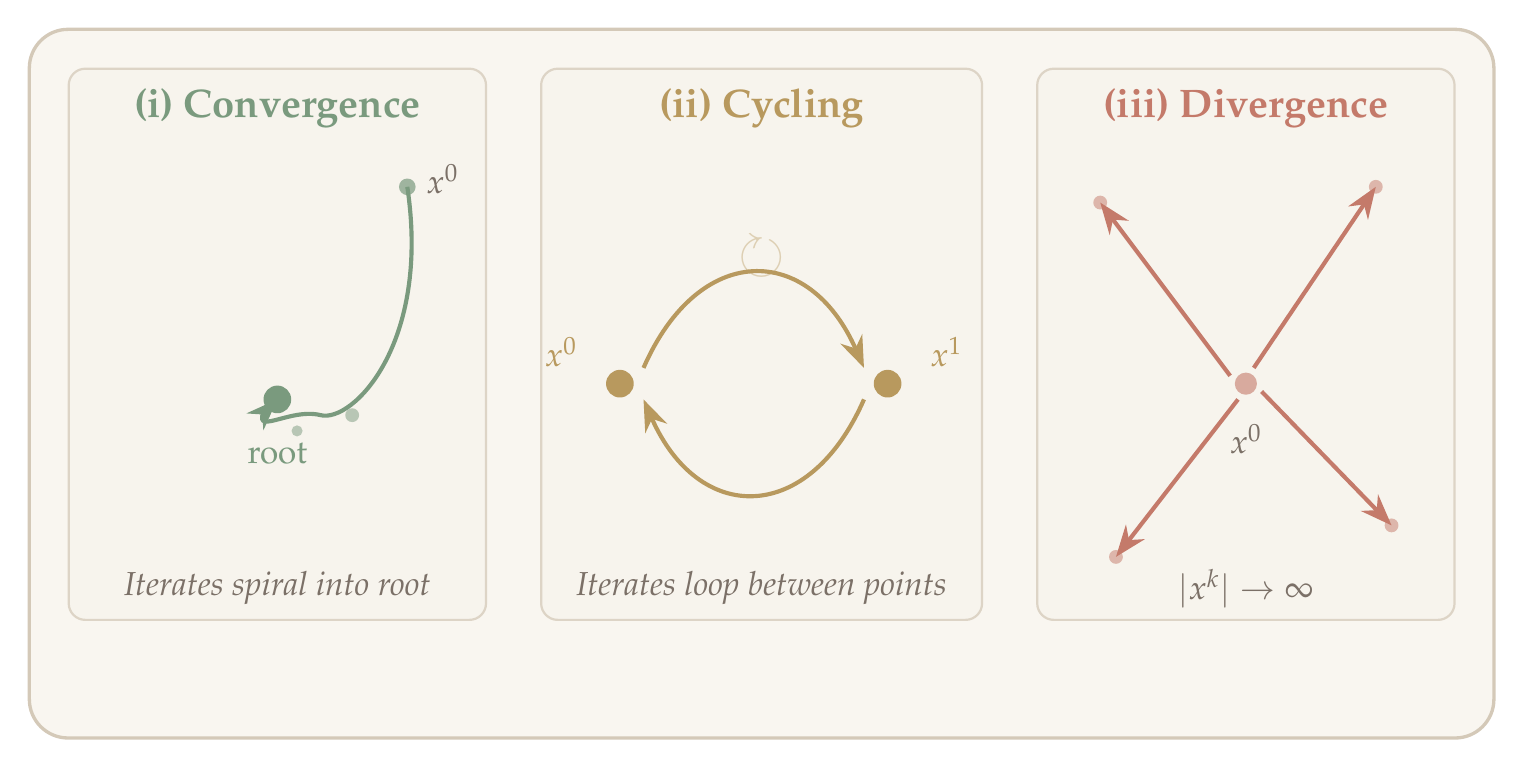
\begin{tikzpicture}[>={Stealth[length=4mm, width=3mm]}, line width=1.5pt]

% Background
\fill[cream, rounded corners=14pt] (-0.3,-1.5) rectangle (18.3,7.5);
\draw[border, line width=1.2pt, rounded corners=14pt] (-0.3,-1.5) rectangle (18.3,7.5);

%% Panel 1: Convergence
\fill[cream!95!border, rounded corners=6pt] (0.2,0.0) rectangle (5.5,7.0);
\draw[border!80, line width=0.8pt, rounded corners=6pt] (0.2,0.0) rectangle (5.5,7.0);
\node[text=sage, font=\Large\bfseries] at (2.85,6.5) {(i) Convergence};

% Target root
\fill[sage] (2.85,2.8) circle (5pt);
\node[text=sage, font=\large, below=6pt] at (2.85,2.6) {root};

% Spiral inward path
\draw[sage, line width=1.5pt, ->]
  (4.5,5.5) .. controls (4.8,3.5) and (3.8,2.5) .. (3.4,2.6)
  .. controls (3.0,2.7) and (2.5,2.3) .. (2.7,2.7)
  .. controls (2.8,2.75) and (2.83,2.78) .. (2.85,2.8);

% Start point
\fill[sage, opacity=0.7] (4.5,5.5) circle (3pt);
\node[text=wmgray, font=\large, anchor=west] at (4.6,5.6) {$x^0$};

% Intermediate points
\fill[sage, opacity=0.5] (3.8,2.6) circle (2.5pt);
\fill[sage, opacity=0.5] (3.1,2.4) circle (2pt);

% Bottom note
\node[text=wmgray, font=\large\itshape] at (2.85,0.4) {Iterates spiral into root};

%% Panel 2: Cycling
\fill[cream!95!border, rounded corners=6pt] (6.2,0.0) rectangle (11.8,7.0);
\draw[border!80, line width=0.8pt, rounded corners=6pt] (6.2,0.0) rectangle (11.8,7.0);
\node[text=rwgold, font=\Large\bfseries] at (9.0,6.5) {(ii) Cycling};

% Two points that cycle
\fill[rwgold] (7.2,3.0) circle (5pt);
\node[text=rwgold, font=\large\bfseries, anchor=east] at (6.8,3.4) {$x^0$};
\fill[rwgold] (10.6,3.0) circle (5pt);
\node[text=rwgold, font=\large\bfseries, anchor=west] at (11.0,3.4) {$x^1$};

% Curved arrows between them (top arc)
\draw[rwgold, line width=1.5pt, ->] (7.5,3.2) .. controls (8.2,4.8) and (9.6,4.8) .. (10.3,3.2);
% Curved arrows between them (bottom arc)
\draw[rwgold, line width=1.5pt, ->] (10.3,2.8) .. controls (9.6,1.2) and (8.2,1.2) .. (7.5,2.8);

% Loop symbol
\node[text=rwgold, opacity=0.4, font=\huge] at (9.0,4.6) {$\circlearrowright$};

% Bottom note
\node[text=wmgray, font=\large\itshape] at (9.0,0.4) {Iterates loop between points};

%% Panel 3: Divergence
\fill[cream!95!border, rounded corners=6pt] (12.5,0.0) rectangle (17.8,7.0);
\draw[border!80, line width=0.8pt, rounded corners=6pt] (12.5,0.0) rectangle (17.8,7.0);
\node[text=terracotta, font=\Large\bfseries] at (15.15,6.5) {(iii) Divergence};

% Center point
\fill[terracotta, opacity=0.6] (15.15,3.0) circle (4pt);
\node[text=wmgray, font=\large, below=5pt] at (15.15,2.8) {$x^0$};

% Arrows going outward
\draw[terracotta, ->, line width=1.5pt] (15.25,3.2) -- (16.8,5.5);
\draw[terracotta, ->, line width=1.5pt] (15.05,2.8) -- (13.5,0.8);
\draw[terracotta, ->, line width=1.5pt] (15.35,2.9) -- (17.0,1.2);
\draw[terracotta, ->, line width=1.5pt] (14.95,3.1) -- (13.3,5.3);

% Scatter dots
\fill[terracotta, opacity=0.5] (16.8,5.5) circle (2.5pt);
\fill[terracotta, opacity=0.5] (13.5,0.8) circle (2.5pt);
\fill[terracotta, opacity=0.5] (17.0,1.2) circle (2.5pt);
\fill[terracotta, opacity=0.5] (13.3,5.3) circle (2.5pt);

% Bottom note
\node[text=wmgray, font=\large] at (15.15,0.4) {$|x^k| \to \infty$};

\end{tikzpicture}
\end{document}
